\title{Cooperative Robot Rolling using Planar Robots to Roll Out of Plane}

\author{David McPherson}

\documentclass[conference]{IEEEtran}

% *** GRAPHICS RELATED PACKAGES ***
%
\ifCLASSINFOpdf
   \usepackage[pdftex]{graphicx}
  % declare the path(s) where your graphic files are
  % \graphicspath{{../pdf/}{../jpeg/}}
  % and their extensions so you won't have to specify these with
  % every instance of \includegraphics
   \DeclareGraphicsExtensions{.pdf,.jpeg,.png,.jpg}
\else
\fi

\usepackage[cmex10]{amsmath}
%\usepackage{flushend}

% *** ALIGNMENT PACKAGES ***
%
\usepackage{array}
\usepackage{mdwmath}
\usepackage{mdwtab}
\usepackage{hyperref}

% *** SUBFIGURE PACKAGES ***
%\usepackage[tight,footnotesize]{subfigure}

% *** FLOAT PACKAGES ***
%
\usepackage{fixltx2e}
\usepackage{stfloats}
%\usepackage{caption}
\usepackage{subcaption}

% *** PDF, URL AND HYPERLINK PACKAGES ***
%
\usepackage{url}

% correct bad hyphenation here
\hyphenation{op-tical net-works semi-conduc-tor}
\usepackage[numbers]{natbib}

\begin{document}

\title{Leveraging Robot Swarms as Planar Manipulation Fingers to Roll Objects out of Plane}

% author names and affiliations
% use a multiple column layout for up to three different
% affiliations
\author{\IEEEauthorblockN{David L. McPherson}
\IEEEauthorblockA{Department of Electrical Engineering and Computer Science\\
University of California at Berkeley\\
Berkeley, California 94720\\
Email: david.mcpherson@eecs.berkeley.edu}
\and
\IEEEauthorblockN{Ronald S. Fearing}
\IEEEauthorblockA{Department of Electrical Engineering and Computer Science\\
University of California at Berkeley\\
Berkeley, California 94720\\
Email: ronf@eecs.berkeley.edu}}


% make the title area
\maketitle

\begin{abstract}
%\boldmath


\end{abstract}

% no keywords

\IEEEpeerreviewmaketitle

\section{Introduction}
The Biomimemtics Millisystems Lab at Berkeley are currently developing a coordinated team of miniature robots to explore an earthquake zone using their RoACH and Zumy platforms. During exploration, hazards may be encountered that cause RoACH robots to stumble and land on their backs. This stable orientation cannot be exited by any simple action of the RoACH's legs. The RoACH is useless in this trapped configuration and considered "lost". Since the RoACH cannot save itself, other robots in the team must be used to recover the RoACH. In this paper, we investigate how a team of mobile robots can roll their fallen comrade back onto its feet. To do so, we cast the multi-robot manipulation problem as a dextrous manipulation problem treating each robot as a separate finger.

In their seminal paper, \citet{rus1995moving} demonstrated techniques for coordinating robots to manipulate furniture.
\citet{sugar2002control} followed up by digging deeper into the controls for such a team of robots manipulating objects in the plane.
This research extends the capabilities of a team of robot manipulators moving in the plane to manipulating objects to roll out of the plane passively.

Rather than add an active flipping arm or mechanism, we will use purely passive kinematics of the pushing robot's shape to manipulate the object.
Shape designs for reorienting objects have been thoroughly explored in the robot hand literature.
\citet{rodriguez2013effector} derived the desired shape for an end effector given a target motion.
\citet{zhang2002gripper} investigated how parallel jaws can reorient objects vertically.
\citet{fearing1986simplified} used cylindrical fingers to allow objects to roll to a new equilibrium.
This work will similarly investigate how designing just the contact shape can result in desired manipulations.

    ...and more citations to come eventually!

\begin{figure}[h!]
\centering
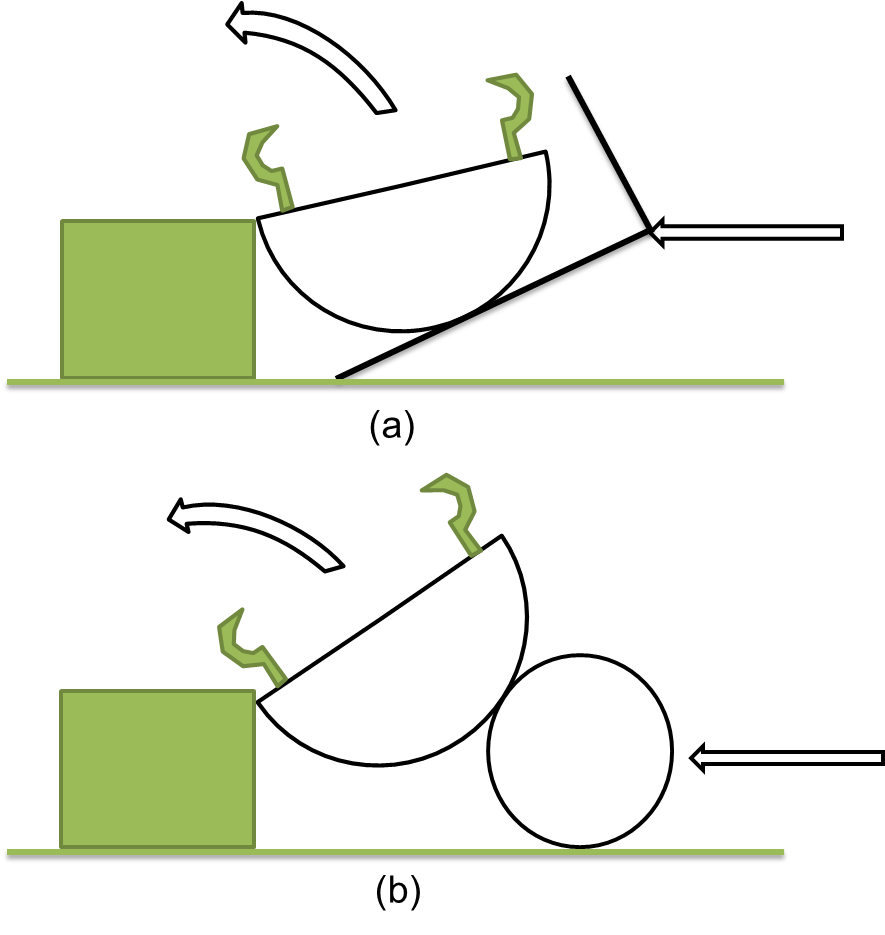
\includegraphics[width=0.3\textwidth]{Overview_Flipping_Strategies.png}
\caption{\label{fig:Over}Overview of Flipping Strategies}
\end{figure}

\section{Mathematical Modeling}
In our model we assume the dead robot is half a cylinder with radius $r_b$. The cylindrical roller is frictionless and has radius $r_a$. The point where the robot contacts the wall or contacts the stop on the backstop RoACH is modeled as a hinge as shown in Figure \ref{fig:math}.

\begin{figure}[h!]
\centering
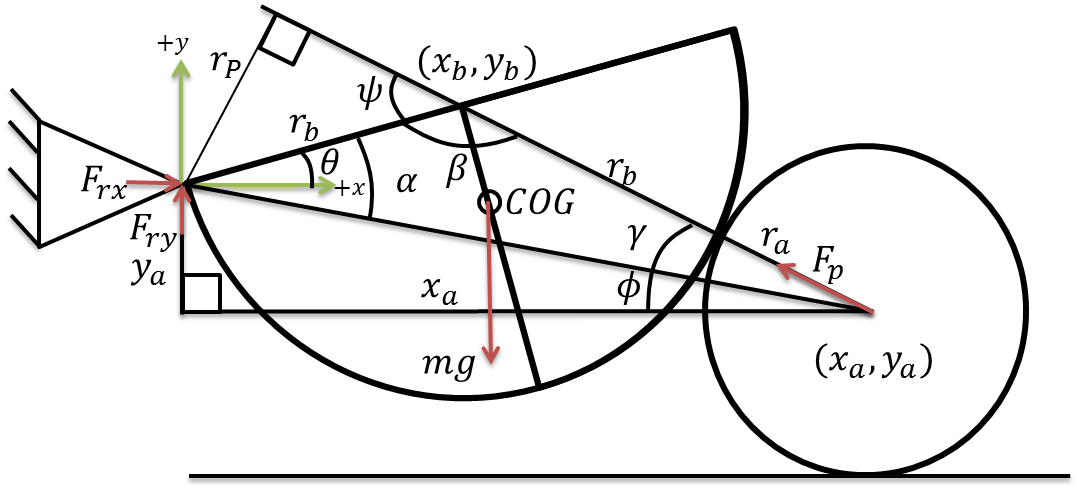
\includegraphics[width=0.3\textwidth]{Principles_of_Manipulation.png}
\caption{\label{fig:math}Freebody Diagram and Dimensions of Cylindrical Plow Flipping Problem}
\end{figure}

Figure \ref{fig:traces} shows the roll angle for the dead robot as the roller plow advances from x=12 down to x=0 from right to left. Each curve represents the roll trace for a different radius of the cylindrical plow. The radius increases from 1 cm in the bottom-most trace up to 4 cm in the top-most trace in steps of 0.3 cm. The point where traces terminate is the point that the cylinder collides with the hinge. The complete red curves represent the roll achieved kinematically as the cylinder continues to slide and make contact. the green subsets of these curves represent where the hinge assumption would be valid due to friction between the dead robot and the wall.

\begin{figure}[h!]
\centering
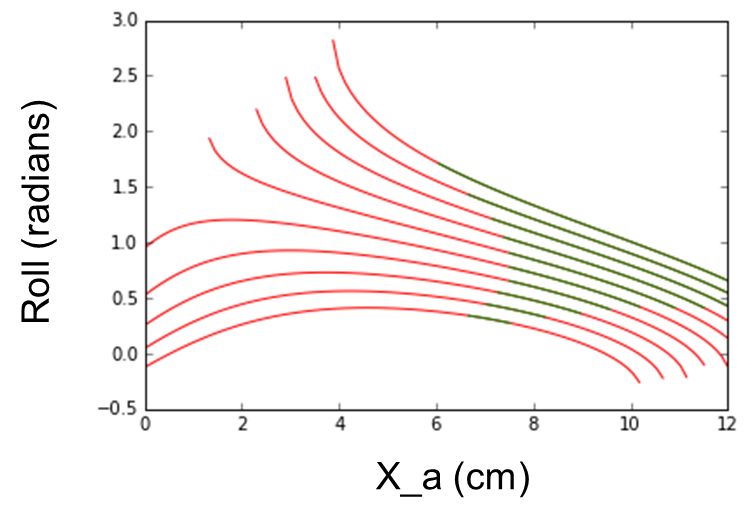
\includegraphics[width=0.3\textwidth]{Flip_Traces.png}
\caption{\label{fig:traces}Roll versus Roller Distance plots for Roller radius varying from 1 cm to 4 cm}
\end{figure}

\section{Experimental Setup}

\begin{figure}[h!]
\centering
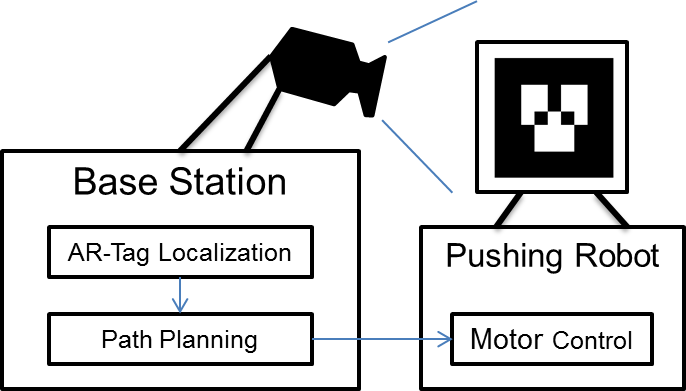
\includegraphics[width=0.3\textwidth]{System_Block_Diagram.png}
\caption{\label{fig:system}Information Flow and Block Diagram of Robot System}
\end{figure}

\section{Experimental Results}
Figure \ref{fig:photos} shows the progression in the robot experiment. First, the pushing robot approaches the dead robot and makes contact. It then pushes the deadbot into the backstop robot, where the dead robot's rim is caught by the stop. The deadbot is then angled slowly upward through constant pushing until it reaches the tipping point where it's center of gravity is over the hinge point. At this point the deadbot tumbles back onto its feet beside/on top of the backstop robot.

\begin{figure}[h!]
\centering
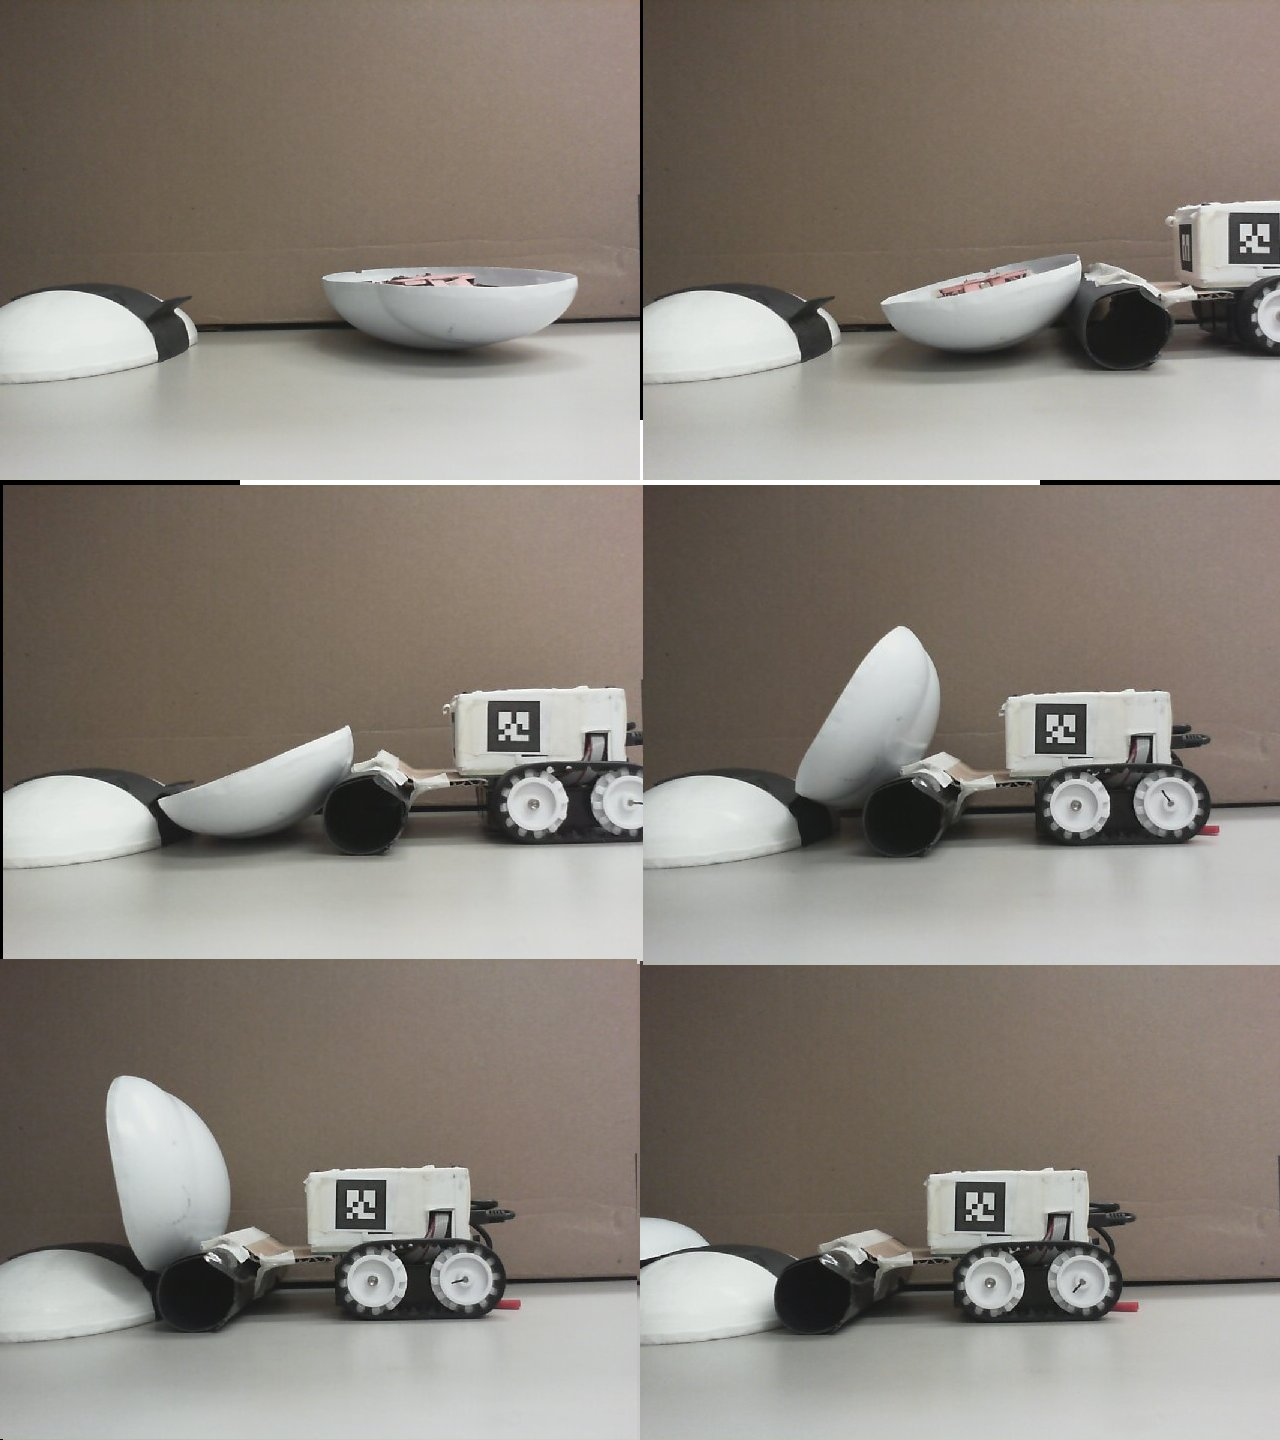
\includegraphics[width=0.3\textwidth]{Photo_Sequence.jpg}
\caption{\label{fig:photos}Photo Sequence of Experimental Flipping}
\end{figure}


\section{Discussion}

\section{Conclusion}



% conference papers do not normally have an appendix


% use section* for acknowledgement
%\section*{Acknowledgment}

% trigger a \newpage just before the given reference
% number - used to balance the columns on the last page
% adjust value as needed - may need to be readjusted if
% the document is modified later
%\IEEEtriggeratref{8}
% The "triggered" command can be changed if desired:
%\IEEEtriggercmd{\enlargethispage{-5in}}

% references section

% can use a bibliography generated by BibTeX as a .bbl file
% BibTeX documentation can be easily obtained at:
% http://www.ctan.org/tex-archive/biblio/bibtex/contrib/doc/
% The IEEEtran BibTeX style support page is at:
% http://www.michaelshell.org/tex/ieeetran/bibtex/
%\bibliographystyle{IEEEtran}
% argument is your BibTeX string definitions and bibliography database(s)
%\bibliography{IEEEabrv,../bib/paper}
%
% <OR> manually copy in the resultant .bbl file
% set second argument of \begin to the number of references
% (used to reserve space for the reference number labels box)

\bibliographystyle{IEEEtranN}
\bibliography{IEEEabrv,david}



% that's all folks
\end{document}
